\documentclass{beamer}
\usetheme{Madrid}
\usecolortheme{default}

\title{Презентація про мене}
\author{Гуцол Альона}
\institute{Спеціальність 111 Математика}
\date{\today}

\usepackage[utf8]{inputenc}
\usepackage[T2A]{fontenc}
\usepackage[ukrainian]{babel}
\usepackage{graphicx}

\begin{document}

% Титульний слайд
\frame{\titlepage}

% Зміст
\begin{frame}
\frametitle{Зміст}
\tableofcontents
\end{frame}

% Розділ: Вступ
\section{Вступ}
\begin{frame}
\frametitle{Вступ}
\begin{itemize}
    \item Мене звати Гуцол Альона.
    \item Я навчаюся за спеціальністю 111 <<Математика>>.
    \item Цікавлюся математикою, інформатикою та програмуванням.
    \item Люблю навчатися, розвивати свої знання та вдосконалювати навички.
\end{itemize}
\end{frame}

% Розділ: Академічні досягнення
\section{Академічні досягнення}
\begin{frame}
\frametitle{Академічні досягнення}
\begin{itemize}
    \item Закінчила школу із золотою медаллю.
    \item Брала участь у конкурсі <<Кенгуру>> у 2017, 2023 та 2024 роках.
    \item Отримала добрий та відмінний результати у математичних конкурсах.
    \item Посіла 2 місце у II етапі Всеукраїнської учнівської олімпіади з математики.
    \item Брала участь у шкільному етапі Міжнародної економічної олімпіади.
\end{itemize}
\end{frame}

% Розділ: Навчальні інтереси
\section{Навчальні інтереси}
\begin{frame}
\frametitle{Навчальні інтереси}

\centering
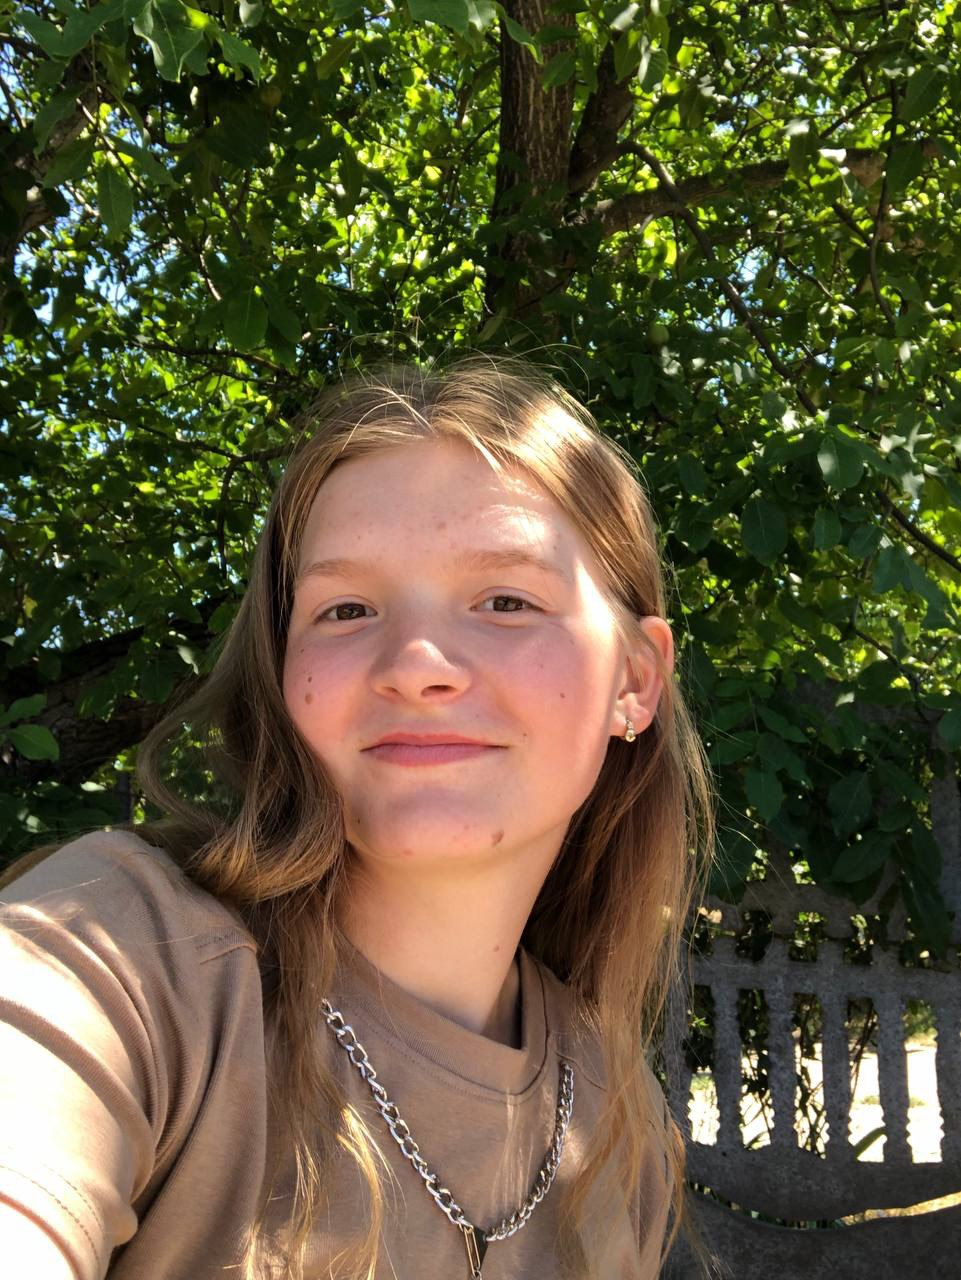
\includegraphics[width=0.32\textwidth]{foto.jpg}

\vspace{0.2cm}

\begin{itemize}
    \item Улюблені предмети: математика, інформатика
    \item Напрямки: програмування, логіка, розв’язування задач
    \item Інструменти: LaTeX, Visual Studio, GitHub
\end{itemize}

\end{frame}


% Розділ: Особисті навички
\section{Особисті навички}
\begin{frame}
\frametitle{Особисті навички}
\begin{itemize}
    \item Комунікабельність
    \item Уміння працювати в команді
    \item Креативність
    \item Відповідальність
    \item Наполегливість у досягненні мети
\end{itemize}
\end{frame}

% Розділ: Хобі та захоплення
\section{Хобі та захоплення}
\begin{frame}
\frametitle{Хобі та захоплення}
\begin{itemize}
    \item Музика
    \item Малювання
    \item Саморозвиток
    \item Цікаві навчальні завдання
\end{itemize}
\end{frame}

% Розділ: Плани на майбутнє
\section{Плани на майбутнє}
\begin{frame}
\frametitle{Плани на майбутнє}
\begin{itemize}
    \item Успішно навчатися за спеціальністю.
    \item Поглиблювати знання з математики та програмування.
    \item Стати хорошим фахівцем у своїй сфері.
    \item Реалізувати себе у професійній діяльності.
\end{itemize}
\end{frame}

% Розділ: Висновок
\section{Висновок}
\begin{frame}
\frametitle{Висновок}
У цій презентації подано коротку інформацію про мене, мої навчальні інтереси,
досягнення, особисті навички, захоплення та плани на майбутнє.
\end{frame}

\end{document}
